\documentclass[11pt]{article}
\usepackage{geometry}
\geometry{letterpaper}

% TODO: roadmap

\usepackage{graphicx}
\usepackage{amssymb}
\usepackage{float}
\usepackage{tabularx}
\usepackage{multicol}
\usepackage{hyperref}
\hypersetup{
    colorlinks,
    citecolor=black,
    filecolor=blue,
    linkcolor=black,
    urlcolor=blue
}

\begin{document}

\newcommand{\PROJECTNAME}{SwarmBot}

\begin{titlepage}
	\newcommand{\HRule}{\rule{\linewidth}{0.2mm}}
	\begin{center}
	\textsc{\LARGE McMaster University}\\[1.5cm]

	\textsc{\Large \PROJECTNAME}\\[0.5cm]
	\textsc{\large Software \& Mechatronics Capstone}\\[0.5cm]

	\HRule\\[0.4cm]
		{\huge\bfseries Hazard Analysis}\\[0.4cm]
	\HRule\\[0.4cm]

	\begin{minipage}[t][][t]{0.5\textwidth}
		\begin{flushleft} \large
			\emph{Authors:}\\
			Victor Velechovsky - \textit{001305263} \\
			Amandeep Panesar - \textit{001431191} \\ 
			Nishanth Balamohan - \textit{001411319}\\
			Gabriel Potter - \textit{001429884}\\
			Taha Mian  - \textit{001417172}\\
		\end{flushleft}
	\end{minipage}
	~
	\begin{minipage}[t][][t]{0.4\textwidth}
		\begin{flushright} \large
			\emph{Professor:} \\
			Dr. Alan Wassyng \\[0.4cm]
			\emph{Teaching Assistants:} \\
			Nicholas Annable \\
			Joshua Barkovic \\
			Spencer Deevy \\
			Viktor Smirnov
		\end{flushright}
	\end{minipage}\\[2cm]

	
\includegraphics[width=0.3\textwidth]{logo.png} \\
	{\large Last compiled on \today}
	\end{center}

\end{titlepage}

\tableofcontents
\listoffigures

\vfill
\vfill
\begin{figure}[htbp]
   \centering
   \noindent\begin{tabularx}{\textwidth}{| >{\centering\arraybackslash}m{0.2\textwidth} | >{\centering\arraybackslash}m{0.2\textwidth} | >{\centering\arraybackslash}m{0.2\textwidth} | >{\centering\arraybackslash}m{0.285\textwidth} |}
   \hline 
   \textbf{Date} & \textbf{Revision} & \textbf{Comments} & \textbf{Author(s)} \\
   \hline
   Jan 18/2019 & 0 & All content added & All authors\\ \hline
   March 7/2019 & 1 & Revised & All authors\\ \hline
   \end{tabularx}
   \caption{Revision History}
\end{figure}
\newpage
\section{Introduction}

\subsection{Project Overview}

\PROJECTNAME \space is a \hyperref[sec:definitions]{swarm} of autonomous robotic cars (\hyperref[sec:definitions]{insect}s) meant to carry out measurements over large areas. For our project, these cars will be measuring temperature, but the idea can be expanded to any number of other quantifiable measurements. Central to our work will be two major components. First, a small motorized car, attached with a temperature sensor, as well as a control unit that allows it to communicate with – and be controlled by – a centralized control unit. Second, a software package that can control a large group (\hyperref[sec:definitions]{swarm}) of these cars, with an algorithm focused on producing reliable, accurate, and fast measurements.\\

Our swarm will aim to cover large areas more quickly and cost-effectively than traditional products. To test the applicability of our project, we will demo it in a small scale area as well as develop a simulation to hypothetically prove the efficacy of the system on a larger scale.\\

Our project will be conducted between Fall 2018 – Winter 2019 for our Engineering Capstone project at McMaster University, under the guidance of Dr. Alan Wassyng. We have four Software Engineering students, and one Mechatronics Engineering student.

\subsection{Document Overview}

This document is intended to be a comprehensive guide to potential hazards that can occur during the
development or use of \PROJECTNAME. Although it attempts to be as comprehensive as possible, there
remains a possibility of other hazards emerging that we did not predict.

Each hazard will contain: a description, a fault tree, and a mitigation plan. This will all discussed
within the system boundary, which is defined in the section \textit{Scope \& Boundary}.
\subsection{Scope and Boundary}
The hazards described below are not only limited to the researcher but can affect the environment and others near the survey area. The damages and potential victims must be addressed and accounted for when analyzing the hazards that may occur during the operation of SwarmBot. Although the system is designed to not harm the user accidents and errors may occur while the insect itself is being guided by the algorithm. The fail safe systems in the communication modules and motor control modules are important in regards to safety but cannot prevent all hazards. Thus the safety actions or fail safe modes are based on the scope of the hazard analysis which includes environmental impact, financial impact, and bodily injury of any body involved to the first degree. 

\subsection{Naming Conventions and Terminology}
\label{sec:definitions}
The following terms and definitions will be used throughout this document:

\begin{itemize}
\item \textbf{System}: The entire software and hardware package - including the cars,
car hardware, control software, and server running the control software
\item \textbf{Swarm}: A large group of objects (in our case, motorized cars) that can communicate and perform acts as a group
\item \textbf{Insect}: A member of the swarm (in our case, a single motorized car)
\item \textbf{Simulation}: The simulation will be used for demo purposes, mainly to show that
the system is valid with a large number of insects.
\item \textbf{Researcher}: A user that is interested in the data that is returned from the survey.
\item \textbf{System Administrator}: A user that controls the parameters of the \hyperref[sec:definitions]{\textbf{swarm}}.
\item \textbf{G.P.S.}: Global Positioning System
\item \textbf{Map}: A 3D visualisation of the data collected by the system.
\item \textbf{API}: Application Programming Interface
\end{itemize}

\section{System}
\subsection{High-Level Design}

SwarmBot contains both hardware components and software components, which can be categorized as
server components or insect components. Each insect will have a car chassis equipped with four motors,
location tracking sensors, and measurement sensors, an RF communication device, and a micro-controller
that functions as the 'brain'.

The server will have a communication protocol, an algorithm to determine where to move each insect,
a data storage component to store measurement data, and a G.U.I. to interact with the user.

The design of the system is covered in detail in the \textit{System Design} document.

\subsection{Financial Losses}
\subsubsection*{Description}
Financial losses could occur either when an insect is damaged or lost, or when an insect causes
damage to the outside world. \\

A major source for insect damage would be water or debris damage. Although the electrical components will be
housed inside the car chassis, adverse conditions could certainly be problematic.

If an insect collides with another insect, or with something in the external world, damage could be
caused to either the insect(s) or the external world. The severity of this hazard is critical since the company is losing funds with every robot damaged or destroyed. The likelihood of this occurring will most likely be low since the insects will operate in an area that has been scouted before hand for any dangers described in the fault tree diagram. 
\subsubsection*{Mitigation Plan}
\textit{Clear Coverage Area}: SwarmBot should only be used in a coverage area that has no
lifeforms or other fragile objects, to minimize the risk of collisions. This includes, for example,
small debris, which could cause problems for the movement of insects.
Ensuring a clear coverage area prior to use is recommended to minimize the risk of collision. 

\textit{Double Check the Coverage Area}: It is important for the proper functionality of \PROJECTNAME
that the coverage area is defined accurately, otherwise insects could travel out of bounds (into deep water),
collide with other insects, or provide measurements that aren't spatially accurate. Ensuring
that the coverage area is properly defined will mitigate such errors.

\textit{Limit Movement Speed}: The maximum speed of the cars can be limited by limiting the voltage
sent to the motors, which could lessen the severity of collisions if they do happen. For development
purposes, velocities of the insects will be limited to 1 m/s.

\subsubsection*{Fault Tree}
\begin{figure}[H]
   \centering
   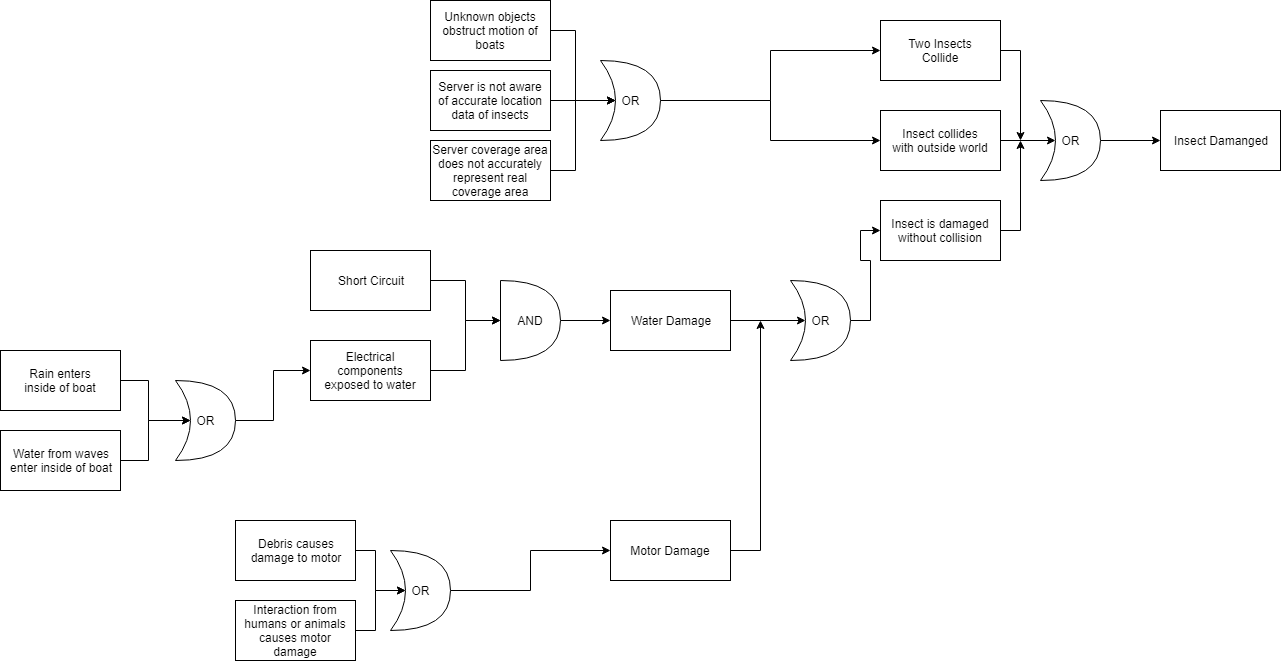
\includegraphics[width=1\textwidth]{Diagrams/Fault Tree - Financial Loss.png} % requires the graphicx package
   \caption{Fault Analysis Tree for \textit{Financial Loss}}
   \label{fig:ft-Air}
\end{figure}

\subsection{Misinformed Policy Decisions}
\subsubsection*{Description}
\PROJECTNAME's measurement data can be used by experts in various fields of study, to inform
policy decisions in the corporate, academic, or political spheres. This, of course, relies on
the assumption of accurate data, so an 'invisible' malfunction in \PROJECTNAME \ 
could lead to misinformed decision making. The likelihood of this hazard is relatively low as well since the research conducted will most likely be double checked in most science journals and is open to be proven wrong. In addition the severity will depend on the inaccuracy of data and on the topic itself. For example, if the SwarmBot was deployed on Mars and found data that leads to scientist to believe an incorrect theory the severity will probably be major vs research that might be less impactful. 

\subsubsection*{Mitigation Plan}
\textit{Cross reference results with a physical model.} In some situations it is possible to
approximate the results of \PROJECTNAME\ using a physical model. If there is a large discrepancy
between the model and swarm, then further investigation is required to ensure the accuracy of
\PROJECTNAME.

\textit{Cross reference results with a second measurement source.} When available, cross referencing
\PROJECTNAME\ with another Coverage Area temperature measuring device is extremely helpful in validating
the accuracy of the system.

\textit{Routinely test the system in known conditions.} If the user has available to them a coverage area
with a known temperature map, the system should be routinely tested in it to validate the
accuracy of the measurement device. Note that both the temperature measurements and the locations
of these measurements should be validated, not simply the temperature measurements themselves.
\subsubsection*{Fault Tree}
\begin{figure}[H]
   \centering
   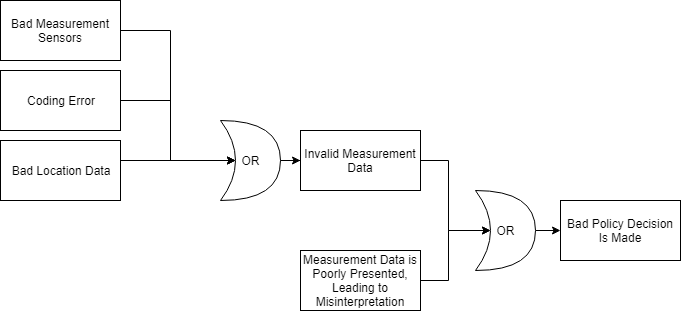
\includegraphics[width=1\textwidth]{Diagrams/Faul Tree - Bad Policy Decision.png} % requires the graphicx package
   \caption{Fault Analysis Tree for \textit{Misinformed Policy Decisions}}
   \label{fig:ft-Air}
\end{figure}

\subsection{Bodily Injury}
\subsubsection*{Description}
Bodily injury may occur during the process of deploying the insect or during the actual survey. One point where bodily injury may occur is when handling the onboard battery on the insect. The improper handling of the battery may lead to a fire and has the potential to seriously harm someone. Injury may also occur when deploying the insect before placing it in the coverage area. The motors on the insect operate at a high R.P.M. and can lead to injury such as bruises on the hand. The severity of this hazard is high since a user should never be harmed when operating the SwarmBot system, however the likelihood of this occurring is low since the insects will all have battery protection circuits and will not move until set to starting position. 

\subsubsection*{Mitigation Plan}
\textit{Overcharge Protection:} The on board battery should be charged for a maximum of three hours.

\textit{Confirm Car Is In Coverage Area:} Double check that the Car is in the Coverage Area before proceeding to run the survey. 

\subsubsection*{Fault Tree}
\begin{figure}[H]
   \centering
   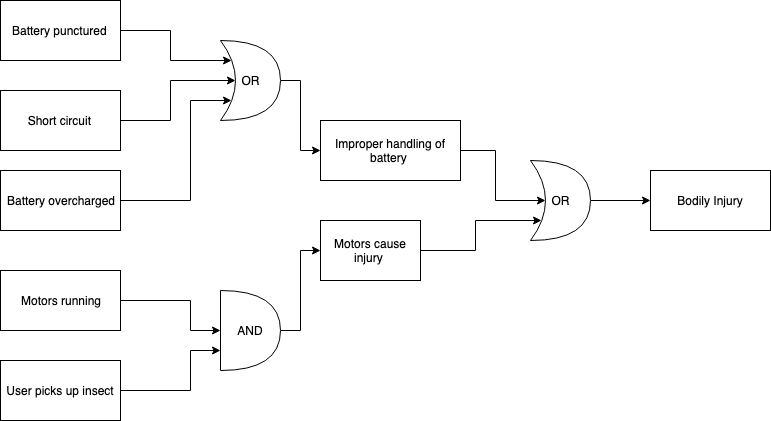
\includegraphics[width=1\textwidth]{Diagrams/FTA-injury.png} % requires the graphicx package
   \caption{Fault Analysis Tree for \textit{Bodily Injury}}
   \label{fig:ft-Air}
\end{figure}

\subsection{Environmental Damage and Habitat Disruption}
\subsubsection*{Description}
Damage to the environment may occur during operation of this device. The following events have the potential to cause environmental damage:
\begin{itemize}
\item Battery leakage
\item Debris from loose components
\end{itemize}
In addition, the following events have the potential to cause habitat disruption:
\begin{itemize}
\item Excessive motor noise
\item Destruction of plant material
\end{itemize}

 The likelihood of this hazard can be minimized substantially by the mitigation plan below. Given the amount of plastic and chemical pollution already present in the environment, this hazard is of medium severity considering the small amount of chemicals actually present in the batteries we are using and the small profile of any parts that could become loose. That being said, we want to avoid contributing to environmental damage as much as possible.

\subsubsection*{Mitigation Plan}
\textit{Secure components:} All components must be reasonably secure to the device to prevent pollution caused by loose part debris. \\
\textit{Small profile:} The cars will have a relatively small profile, minimizing plant destruction and eliminating the need for large motors that may generate excessive noise. \\
\textit{Sealing and internalization of components:} All electronic components including the battery compartment will be sealed and located within the insect. This will prevent a ruptured battery from leaking into the environment.

\subsubsection*{Fault Tree}
\begin{figure}[H]
   \centering
   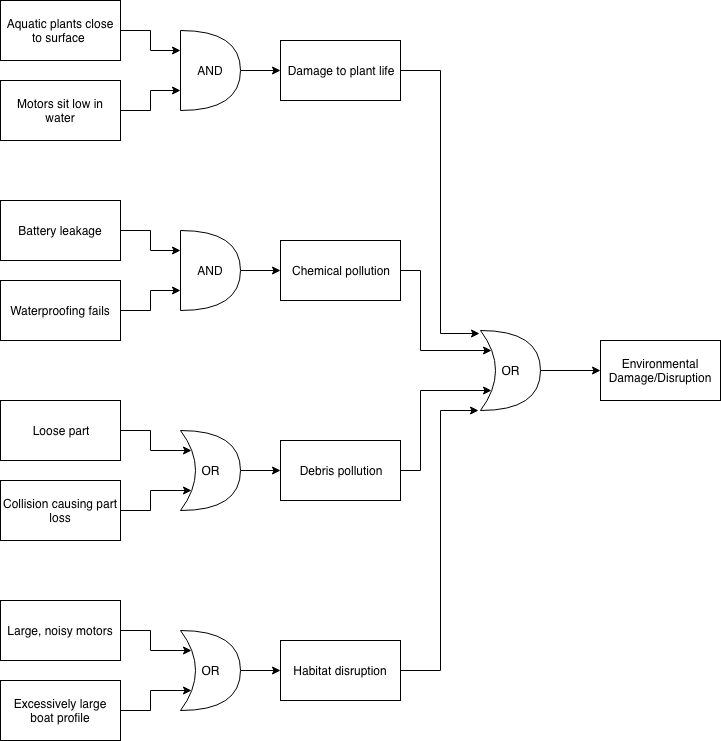
\includegraphics[width=1\textwidth]{Diagrams/environmental_hazard_fta.png}
   \caption{Fault Analysis Tree for \textit{Environmental Damage and Habitat Disruption}}
   \label{fig:ft-Environment}
\end{figure}

\subsection{Loss of Time}
\subsubsection*{Description}
If the system breaks down during operation, the user can experience a severe loss of time. Mitigations include anything
that can improve system reliability.

\begin{itemize}
\item Insect retrieval from coverage area
\item Delayed component delivery time
\item Damaged insect requiring repair
\end{itemize}

The severity of this hazard is also dependent on the application and or research being conducted using the SwarmBot. Loss of time due to the abnormal scenario of the insects being lost and having to be retrieved manually will cause a major delay. The delay might affect the data being collected such as checking the humidity at the north pole during different hours of the day. In addition, the current number of insects available to the user currently is maxed out at three and if a time sensitive application needs to use SwarmBot the delay in receiving parts will directly affect research. The likelihood of both the insect needing to be retrieved and need of components will be relatively low since the insects are supposed to return to the start position if any error occurs, and parts will be more accessible once bought in bulk. 

\subsubsection*{Mitigation Plan}
\textit{Insect Start Point:} Prepare a system where in the case of a damaged insect, it is able to be manually driven to a start point. \\
\textit{Order Early:} Order the components as early as possible and anticipate faulty parts when ordering. \\
\textit{Modular components:} All components must be operational individually, they will be tested to validate its functionality. When integrated with other units there will be a decreased chance of damage to the components. The components will also be integration tested to make sure the components function together. \\

\subsubsection*{Fault Tree}
\begin{figure}[H]
   \centering
   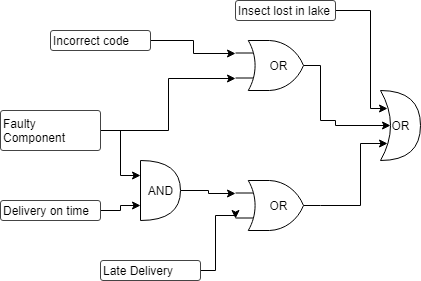
\includegraphics[width=1\textwidth]{Diagrams/Fault Tree - Time Loss.png}
   \caption{Fault Analysis Tree for \textit{Loss of Time}}
   \label{fig:ft-Time}
\end{figure}

\end{document}
